\documentclass[a4paper, 12pt, twoside]{article}
\usepackage[utf8]{inputenc}		% LaTeX, comprend les accents !
\usepackage[T1]{fontenc}		
\usepackage[french]{babel}
\usepackage{lmodern}
\usepackage{ae,aecompl}
\usepackage[top=2.5cm, bottom=2cm, left=3cm, right=2.5cm,headheight=15pt]{geometry}
\usepackage{graphicx}
\usepackage{eso-pic}	% Nécessaire pour mettre des images en arrière plan
\usepackage{array} 
\usepackage{amsmath}
\usepackage{hyperref}
 \usepackage{array}
 \usepackage{amsmath,amsfonts,amssymb}
\usepackage{lastpage}
\definecolor{bleuleger}{RGB}{0,0,200}
\newtheorem{definition}{Définition}
\usepackage{listings}
\usepackage{titlesec}
\setcounter{secnumdepth}{4}
\titleformat{\paragraph}
{\normalfont\normalsize\bfseries}{\theparagraph}{1em}{}
\titlespacing*{\paragraph} {0pt}{3.25ex plus 1ex minus .2ex}{1.5ex plus .2ex}

%%%%%%%%%%%%%%%%%%%%%%%%%%%%%%%%%%%%%%%%
%    Page de garde (Pagedegarde.tex)   %
%%%%%%%%%%%%%%%%%%%%%%%%%%%%%%%%%%%%%%%%
% Dorian Depriester, 2014

\makeatletter
\def\@ecole{école}
\newcommand{\ecole}[1]{
  \def\@ecole{#1}
}

\def\@entreprise{Nom de l'entreprise}
\newcommand{\entreprise}[1]{
  \def\@entreprise{#1}
}

\def\@datedebut{\today}
\newcommand{\datedebut}[1]{
  \def\@datedebut{#1}
}


\def\@datefin{\today}
\newcommand{\datefin}[1]{
  \def\@datefin{#1}
}



\def\@specialite{Spécialité}
\newcommand{\specialite}[1]{
  \def\@specialite{#1}
}

\def\@ED{\'{E}cole Doctorale}
\newcommand{\ED}[1]{
  \def\@ED{#1}
}

\def\@doctorat{Doctorat}
\newcommand{\doctorat}[1]{
  \def\@doctorat{#1}
}

\def\@adresse{Adresse}
\newcommand{\adresse}[1]{
  \def\@adresse{#1}
}

\def\@directeur{directeur}
\newcommand{\directeur}[1]{
  \def\@directeur{#1}
}

\def\@encadrant{encadrant}
\newcommand{\encadrant}[1]{
  \def\@encadrant{#1}
}
\def\@membrea{Membre}
\newcommand{\membrea}[1]{
  \def\@membrea{#1\\}
}



\def\@juryb{}{}{}
\newcommand{\juryb}[3]{
  \def\@juryb{#1,	& #2	& #3\\}
}
\def\@juryc{}{}{}
\newcommand{\juryc}[3]{
  \def\@juryc{#1,	& #2	& #3\\}
}
\def\@juryd{}{}{}
\newcommand{\juryd}[3]{
  \def\@juryd{#1,	& #2	& #3\\}
}
\def\@jurye{}{}{}
\newcommand{\jurye}[3]{
  \def\@jurye{#1,	& #2	& #3\\}
}
\def\@juryf{}{}{}
\newcommand{\juryf}[3]{
  \def\@juryf{#1,	& #2	& #3\\}
}
\def\@juryg{}{}{}
\newcommand{\juryg}[3]{
  \def\@juryg{#1,	& #2	& #3\\}
}
\def\@juryh{}{}{}
\newcommand{\juryh}[3]{
  \def\@juryh{#1,	& #2	& #3\\}
}
\def\@juryi{}{}{}
\newcommand{\juryi}[3]{
  \def\@juryi{#1,	& #2	& #3\\}
}
\makeatother

\newcommand\BackgroundPic{%
	\put(0,0){%
		\parbox[b][\paperheight]{\paperwidth}{%
			\includegraphics[height=0.45\paperheight]{bordure.png}%
			\vfill
		}
	}
}
\newcommand\EtiquetteThese{%
	\put(0,0){%
		\parbox[t][\paperheight]{\paperwidth}{%
			\hfill
			%\colorbox{blue}{		
				\begin{minipage}[b]{2em}
					
\includegraphics[width=4.0\textwidth]{logo_miage.png}\\					
					%\centering\Huge\textcolor{white}{M\\I\\A\\G\\E\\}
					\vspace{0.2cm}
				\end{minipage}
			%}
		}
	}
}

\makeatletter
\newcommand{\pagedegarde}{
\newgeometry{top=2.5cm, bottom=1cm, left=2cm, right=1cm}
\AddToShipoutPicture*{\BackgroundPic}
%\AddToShipoutPicture*{\EtiquetteThese}
  \begin{titlepage}
  \centering
      
\includegraphics[width=0.6\textwidth]{logo_Paris_Nanterre_couleur_RVB.png}
      \hfill
      $\ $\\
      %
\includegraphics[width=0.20\textwidth]{logo_entreprise.png}\\
    \vspace{1cm}
      {\Large Licence MIAGE}\\
    \vspace{1cm}
      {\huge 
      	{\bfseries Mémoire Stage Licence 3 MIAGE CLASSIQUE}\\
    \vspace{0.5cm}}
      	$\ $\\
    \vspace{1cm}
   		
    \vspace{1cm}
    	{\huge\color[rgb]{0,0,1} \bfseries{\@title}}\\
    \vspace{0.5cm}
    %{\bfseries Entreprise d'accueil : \@entreprise}\\
    {\bfseries Stage réalisé du \@datedebut\ au \@datefin}\\
    %	{\Large{\bfseries Spécialité doctorale ``\@specialite''}}\\
    \vspace{2cm}
    $\ $\\
    \vspace{0.5cm}
    $\ $\\
    \vspace{0.5cm}
    %	le \@date \\
    \vfill
     %  {\LARGE \color[rgb]{0,0,1} \bfseries{\@title}} \\
    %\vfill
      %  Directeur de thèse : {\bfseries \@directeur}\\
       % Co-encadrant de thèse : {\bfseries \@encadrant}\\
    %\vfill
	\begin{tabular}{>{\bfseries}lll}
		\large Avi ASSAYAG\\
		\vspace{0.15cm}\\
		%\@membrea
		%\@jurye
		%\@juryf
		%\@juryg
		%\@juryh
		%\@juryi
	\end{tabular}
	%
\includegraphics[width=0.20\textwidth]{logo_entreprise.png}\
	\vfill
	
	%\@adresse
  \end{titlepage}




\restoregeometry  
}



\author{Avi ASSAYAG}
\title{Implémentation d'algorithmes pour modèles de jeu stochastiques}
\entreprise{Université Paris Nanterre}
\fonction{Développeur Junior Python }
\datedebut{23 mars 2020}
\datefin{22 mai 2020}

\date{25 mai 2020}
\jurya{M. François Delbot}{Maître de conférences}{Responsable du L3 MIAGE}

\juryb{M. François Delbot}{Maître de conférences}{Tuteur enseignant}
%Le titre de votre enseignant référent est soit Maître de conférences, soit Professeur des universités. Si vous aves un doute, demandez moi. 

\juryc{M. Emmanuel Hyon }{Maître de conférences}{Maître de stage}
%Demandez à votre maître de stage quel est son poste. Par exemple, directeur du système d'information, chef de projet, responsable d'équipe etc...

%\juryd{M. Prénom Nom}{poste de votre maître de stage}{Maître de stage}
%Ajouter le juryd si votre maître de stage viens accompagné d'un collègue.

\begin{document}
\pagedegarde


%placer vos remerciements ici
\section*{Remerciements}
Merci à Monsieur Hyon, maitre de conférence à l'Université de Nanterre et chercheur dans l'equipe SYSDEF du Lip6 , d'avoir accepter le poste de tuteur pour mon stage de Licence 3 MIAGE. Grâce a son accompagnement personnel j'ai pu solidifier mes compétences algorithmiques (Java et Python) mais aussi découvert d'autre aspect de la programmation linéaire.
\newline 

Cette opportunité n'a été seulement possible que par la collaboration de Monsieur Emmanuel Hyon, mon tuteur ainsi que Monsieur François Delbot, responsable de la Licence 3, et les remercie de leur patience , de leur encouragement et de le encadrement tout au long de ce stage.
\newline

Merci aussi aux autres professeurs qui ont contribué tout a long de l'année à parfaire toutes nos compétences autant sur le plan théorique que techniques. \newline

Enfin je tiens aussi à remercier mes relecteurs qui ont permis de rendre ce mémoire aussi précis et grammaticalement correct  , mais aussi d'être un document accessible et utile à tous si un jour vous décider de vous lancer dans le même sujet que moi.
\newpage

%La table des matières
\tableofcontents
\newpage

\section{Introduction}
Pendant ces semaines de stage, nous allons essayez d'implémenter des algorithmes pour résoudre des modèles de jeux stochastiques, plus précisément des jeux  de gain à somme nul (que nous représenterons sous forme bimatricel). \newline

L'objectif est dans un premier temps de concevoir une modélisation informatique de ces jeux puis dans un second temps implémenter un ou des algorithmes permettant de résoudre ces jeux.  \newline

Pour parfaire à ces attentes, nous allons utilisé le langage \textsf{Python}, non utilisé durant le cursus scolaire actuel, le solveur \textsf{Gurobi}, que nous utiliserons afin de résoudre des programmes linéaires et pour l'orienté objet \textsf{Python} et la plateforme \textsf{GitHub}, l'hébergeur de code, pour avoir accès a tout les codes sources, document qui m'ont aidé a réaliser ce stage. \newline

L'utilisation de \textsf{GitHub} n'était pas obligatoire, mais elle était plus que judicieuse afin que mon tuteur \underline{\textsf{Mr Emmanuel Hyon}} puisse avoir accès en temps réel à mon code afin de m'orienter si je m'écarte du sujet. C'est donc à son initiative que nous avons utilisé \textsf{Github} tout au long de ce stage. \newline

Dans les chapitres qui suivront nous allons expliciter différents concepts relatifs aux \textsf{ modèles stochastiques} (notamment le principe même de la théorie des jeux) mais aussi les outils utilisés ; comment les installer et les utiliser. \newline

Enfin nous tenterons de rédiger et de résoudre différents modèles de \textsf{jeu à sommes nulles} , c'est a dire un jeu ou le gain d'un des acteurs représente la perte exacte des autres acteurs de ce jeu, mais nous l'expliquerons en détails dans une prochaine section [4.3.1].  \newline

Les \textsf{jeux à sommes nulles} sont nombreux vous connaissez surement le jeux \textsf{pierre-feuille-ciseau}, mais aussi le \textsf{dilemme du prisonnier}, ou encore le \textsf{dilemme du voyageur} et tant d'autres. \newline

Dans les semaines de ce stage nous avons décider d'implémenter un \textsf{jeu à somme nulle} moins connu que les précédents mais tout aussi intéressant il s'agit : du jeu  \textsf{ "Matching Pennies"}\newline

Enfin nous étudierons plus en profondeurs qu'est ce que sont les jeux stochastiques mais surtout comment définir un modèle informatique (en \textsf{python}) et sa résolution grâce à la programmation linéaire (via \textsf{gurobi}).

\newpage
\section{Contexte du Stage}
Durant le seconde semestre de la troisième année de notre licence Miage (S6), nous sommes tenus d'effectuer un stage en entreprise d'une durée minimum de 10 semaines. Pour cela j'ai donc recherché activement depuis le mois de février une entreprise prête a m'accueillir en stage afin de me former et de compléter mes connaissances. En attendant des réponses positives, j'avais quand même envisagé d'effectuer une demande (avec l'accord de mon professeur référant \textsf{Monsieur Delbot} au près de l'un de enseignants de l'université en cas de refus de candidatures potentielles. \newline

Avec la crise sanitaire que nous traversons et en l'absence de réponse positive la direction de la formation à fait tout son possible pour que le stage se passe dans les meilleurs conditions possible (tant sur le plan sanitaire que sur le plan logistique) et ainsi  j'ai pu obtenir un sujet de stage, dirigé par mon professeur \textsf{Monsieur Hyon} au seins de la faculté.
\subsection{Présentation de l'entreprise}
L'université Paris Nanterre, de nom officiel \textsf{Paris X} est une université française fondé le 20 Octobre 1964 et spécialisé dans les sciences économiques et sociales, le droit, la psychologie et l'informatique. Elle se situe à Nanterre (92000) , à deux pas de l'un des centre économique de Paris , La Défense.  \newline

Le campus s'étend sur plus de 32 hectares et compte plusieurs restaurants (dans le restaurant universitaire Croos), de nombreux espaces verts , un terrain d'athlétismes, des cours de tennis et une piscine.  On y dénombre environs 35 000 étudiants (sans compter ceux inscrit à distance) repartis dans 8 UFR (Unité de Formation et de Recherche) et 5 instituts, pour un un total d'environs 2 200 enseignants chercheurs (respectivement 1800 et 400).
\begin{center}
\begin{figure}[h]
\centering

\includegraphics[scale=1.3]{campus.jpeg}
\caption{Le campus de Nanterre}
\end{figure}
\end{center}

Comme nous l'avons expliqué l'Université est organisé autours de 8 UFR : \vspace{0.4 cm}
\begin{itemize}
\item UFR Langues et cultures étrangères \textsf{(LCE)} 
\item UFR Littérature, langages, philosophie et arts du spectacle \textsf{(PHILLIA)}
\item UFR Droit et science politique \textsf{(DSP)}
\item UFR Sciences psychologiques et sciences de l'éducation \textsf{(SPSE)}
\item UFR Sciences sociales et administratives \textsf{(SSA)}
\item UFR Sciences et techniques des activités physiques et sportives \textsf{(STAPS)}
\item UFR Systèmes industriels et techniques de communication \textsf{(SITEC)}
\item UFR Sciences économiques, gestion, mathématiques et informatique \textsf{(SEGMI)} 
\end{itemize}
\subparagraph*{}{Évidemment il subsiste une hiérarchie au seins l'Université, à sa tête on y trouve Monsieur \textsf{Jean-François Balaudé} (depuis 2012) puis chaque UFR à un président et chaque parcours universitaire (mathématiques, informatique, droits, économie, gestion etc...)  a un responsable par niveau (licence et master) et par voie d'études (classique ou apprentissage).}

\subsection{Présentation du service et de l'équipe}
Effectuant mon stage à l'université de Nanterre et étant étudiant en troisième année de licence MIASHS parcours MIAGE, il était logique d'effectuer mon stage au seins de l'UFR \textsf{SEGMI} (Sciences économiques, gestion, mathématiques et informatique). \newline

A sa direction on trouve Monsieur \textsf{Yann Demichel}, enseignant chercheur mathématique au seins de l'université de Nanterre (Paris X) puis différents responsables par formation. Concernant le parcours MIAGE, nous avons Monsieur \textsf{Jean-François Pradat-Peyre} enseignant chercheur et responsable du département mathématique et informatique puis respectivement Monsieur \textsf{Pascal Poizat} et Madame \textsf{Marie Pierre Gervais} responsable du master MIAGE classique et alternance. Quant aux licences elles sont gérer respectivement par Monsieur \textsf{François Delbot} et Madame \textsf{Sonia Saadaoui} responsable de la licence MIAGE classique et alternance. \newline

Quant à mon tuteur Monsieur \textsf{Emmanuel Hyon} il est enseignant chercheur mais aussi   maitre de conférence à l'université de Nanterre (Paris X) depuis 2004 et nous à donner cours d'algorithme et programmation C lors du premier semestre de la licence MIAGE. \newline

Travaillant principalement au LIP6 (Département Desir ) en recherche opérationnel (RO) et sur modélisation mathématique et informatique à l'université de Nanterre (Paris X) il parrait logique de choisir comme thème de stage : \textsf{Implémentation d'algorithmes pour modèles de jeux stochastiques}. \newline

Au vue de la situation peu évidente et inhabituelle, et dans le but de préserver un maximum notre santé j'ai effectué mon stage à domicile donc sans la présence de mon tuteur, ce qui aurai rendu le stage encore plus intéressant et plus évident à gérer (d'un point de vue logistique et pour des questions potentielles). Pour remédier à cela et à l'initiative de Monsieur \textsf{Hyon} mon tuteur, nous avons mis en place un lien \textsf{GitHub} mais aussi un rendez vous téléphonique hebdomadaire en début de semaine permettant de faire le point, de poser mes questions, de me donnez les axes que je devais améliorer ainsi que les points sur lesquels je devais travailler pour la semaine à venir.  

\subsection{Mission proposée}
Ainsi il m'à été confié de modéliser un jeu stochastique sur un point de vue informatique (via \textsf{pyhton}) mais surtout de trouver un moyen, par un algorithme de le résoudre c'est à dire de trouver la solution la plus optimale (nous reviendrons plus en détails dans les sections futures cf [4.2], [4.3]). \newline

Pour cela j'ai du apprendre les bases, la syntaxe et le fonctionnement du langage \textsf{python} mais aussi me familiariser avec le concept orienté objet (déjà étudié durant mon cursus avec \textsf{C++} et \textsf{Java}) sur un nouveau langage : \textsf{python}. \newline

De plus j'ai du apprendre utiliser un solveur mathématique \textsf{gurobi} afin de trouver la solution optimale , autrement maximiser la fonction objective (représentant la solution du jeu en question cf [RO]). \newline

Ainsi tout ça à eu pour but de me permettre de modéliser et résoudre tout d'abord le jeu de \textsf{Matching Pennies}, un jeu bimatriciel à somme nulle puis dans un second temps la modélisation et la résolution d'un jeu bilatéral. \newline

Aimant les mathématiques et l'informatique depuis jeune le sujet de ce stage me correspond parfaitement et complaît mon envie de poursuivre mes études avec un master MIAGE.
\subsection{Cahier des charges}
Il m'est un peu compliqué de donner des dates exactes et précise de chaque tâches à réaliser ou effectués mais je peux énumérer la liste des charges à accomplir : \vspace{0.4 cm}
\begin{itemize}
\item Mise en place d'un lien \textsf{GitHub} (pour avoir accès en temps réel au codes sources mais aussi au rapport)
\item Installation de \textsf{python} (version 3.8)
\item Apprentissage du langage \textsf{python} et des propriétés orienté objet (POO)
\item Installation du solveur \textsf{gurobi}
\item Apprentissage de la syntaxe  \textsf{gurobi} et du module \textsf{gurobi} pour la modélisation des jeux (de tout type)
\item S'informer sur les concepts fondamentaux de la théorie de jeux
\item Définir les notions de jeu bimatriciel, jeu stochastique, stratégie, gain
\item Approche mathématique de \textsf{l'équilibre de Nash}
\item Création d'un objet "Jouet" en \textsf{python}
\item Modéliser et résoudre un programme linéaire (biere.py) 
\item Modéliser et résoudre le jeu \textsf{Matching Pennies}
\item Modéliser et résoudre un jeu \textsf{stochastique bilatéral}
\item Rédaction du mémoire pour la soutenance de stage (semaine du 25 mai)
\end{itemize} 

\subparagraph*{}{Ainsi pendant 10 semaines et ce depuis le 23 mars, je travaille quotidiennement de le but d'implémenter des algorithmes pour modèles de jeux stochastiques.}
\newpage

\section{Outils utilisés}
\subsection{GitHub}
\texttt{Github} est un service d'hébergement web (un peu comme une sorte de Drive) et de gestion de développement de logiciel lancé en 2008. Ce dernier est codé principalement en Ruby et Erlang par différents programmeurs : Chris Wanstrath, PJ Hyett et Tom Preston-Werner.\newline

Aujourd'hui cette plateforme compte plus de 15 millions d'utilisateurs et enregistre environ 40 millions de dépôts de fichiers,
se plaçant donc en tête du plus grand hébergeur source code mondial. \newline

Le fonctionnement de Git est assez simple, on créer un répertoire (un référentiel / requisitory) dans lequel on va stocker tout les fichiers que l'on désire et on peut soit rendre l'accès publique (au quel cas tout le monde peut rejoindre et consulter ces fichiers) ou alors le  restreindre en accès privé (au quel cas c'est le créateur qui décide quels seront les collaborateurs ayant droit de consultation des fichiers). \newline

Ensuite cela s'agit comme une sorte de réseau constitué de branches (branch) où chaque branches représentent un collaborateur ainsi que la master qui correspond au créateur du référentiel. \newline

Une des caractéristiques de Git repose sur le fait que c'est un outil de verisonning (gestion de version) est donc permet de si le fichier à été modifié; si oui par qui et quand a eu lieu la modification et quel fichiers ont été affectés. Cela permet notamment de pouvoir faire
des travails de groupe sur le même sujet (un site ou une application par exemple) où chacun doit travaillé sa partie mais nécessite les parties des autres membres du groupes (mis à jours régulièrement). \newline
Évidemment toutes les étapes (initialisation, dépôts, fusion et clonage) se font a l'aide de lignes de commandes sur le terminal (en bash) que j'expliquerai un peu plus loin ainsi que les commandes principales pour chaque étapes.\newline

\subsubsection{Initialisation}
Pour créer un projet il suffit d'aller sur le site  https://github.com/ puis Repositories --> New et remplir les informations données avant de valider. Ensuite pour initialiser le Git (et que la branch master existe; elle sera crée automatiquement a l'instantaciation du projet) il faut se placer dans le dossier (en ligne de commande cd) et tappez :  git init \newline

Ensuite  il faudra taper :  git remote add origin < lien donnée par git hub >  puis  git push –u origin master  qui respectivement créerons le répertoire du projet et ensuite la zone de dépôt.

\subsubsection{Branches}
Comme nous l'avons dit plus haut le projet est contenu dans la branche principale la master et grâce à des copies de branches le projet acquiert une plus grande flexibilité qui permet d'incrémenter au fur et mesure le projet. \newline

Pour ajouter une branche il suffira simplement de taper  git branch < nom de la branche >  et pour supprimer une branche il faut rajouter l'option -d a la commande soit :  git branch -d < nom de la branche >.\newline

Pour changer de branche (afin d'effectuer un dépôt ou autre) il faudra taper :  git checkout < nom de la branche >   et enfin pour visualiser l'ensemble des branches existantes on devra taper :  git branch .

\subsubsection{Dépôt et mises à jours}
Avant toute chose il faut savoir sur quelle branche déposer le fichier puis il faudra taper les commandes suivantes pour les ajouter  au fichier :  git add < nom des fichier >  (ou * pour tout ajouter) puis  git commit -m message  et enfin pour finir git push origin < nom de la branche>. \newline
Pour récupérer des modifications faites sur le projet il suffit à l'inverse de taper : 
 git pull origin master.
 
\subsubsection{Clonage}
Une fois les autres branches (celles des différents collaborateurs) crées il faut juste qu'il copie le lien du git pour pouvoir travailler dessus et effectuer les futurs dépôts. En premier lieu il faudra taper :  git clone < lien du git >  puis effectuer la commande git pull origin master  pour récupérer les fichiers de la branche master et enfin faire les commandes relatives au dépôt (vu plus haut).

\subsection{Python}
Python est un langage de programmation à part entière dont la première version fut développe par \textsf{Guido van Rossum} et lancé en 1991. Ce langage est facile d'utilisation et ne possède pas forcément de syntaxe particulières seulement une indentation permettant au compilateur intégré de suivre les blocs d'instructions. \newline

Ce langage permet donc une multitude de possibilité de code mais aussi d'action puisqu'il existe des bibliothèques déjà implémentés et il suffira seulement des les utiliser comme bon nous le semble (par exemple Matplotlib ou encore Networkx etc...). Malheureusement Python n'est pas le langage le plus rapide d'exécution contrairement au C ou C++ et Java mais il permet tout de même d'accéder à des fonctionnalités que d'autres langages ne peuvent proposer. \newline

Contrairement au C, Python admets des types sophistiqués supplémentaires tel que les \textsf{Listes}, les \textsf{Dictionnaires}, les \textsf{Sets} et les \textsf{Tuples}. Il en va de soit que les types primitifs sont aussi présent \textsf{int,float,double,boolean etc..}. Mais le réel avantage du langage repose sur le fait que l'on ne se soucie pas du type de retour d'une fonction ni de la déclaration du type du paramètre ainsi que le langage admet la possibilité d'être orienté objet. \newline

Python est un langage interprété et donc n'a pas besoin de passer pas un compilateur comme GCC (GNU Complier Collection), tout se fait directement sur la console une fois l'environnement installé. \newline

Quant à l'installation de Python, cette dernière est assez simple; il suffit d'aller sur le site officiel et télécharger la version en question (aujourd'hui version 3.8.2) et ensuite de l'installer. Il existe différentes méthodes d'activation du langage, qui représente chacune l'environnement de la machine (Windows, Mac OS ou encore Linux).\newline

A savoir que sur Mac Os et Linux, Python est déjà préinstallé et il faudra peut être seulement mettre à jours la version qui pourrai être obsolète ou dépassé.

\subsubsection{Procédure d'installations de Python} 
\paragraph{Méthode packages}{Pour cela il faut allez télécharger les packages en question sur le site officiel de Python puis les interpréter c'est dire ouvrir la console (terminal python) et demander à python d'exécuter le fichier \textsf{.py} en question via la commande :}
\begin{verbatim}
python setup.py install
\end{verbatim} 

\paragraph{Méthode module Pip} {Il s'agit d'une des méthodes les plus simple, après avoir téléchargé les packages Python sur le site, on installe tout les modules externes (pip , Django etc ...)  que l'on pourrai avoir besoin d'utiliser par la suite via le terminal : }
\begin{verbatim}
pip install <nom_module>
\end{verbatim}

\paragraph{Environnement virtuel python}{On parle d'environnement virtuel pour certaines utilisation bien propre à \textsf{python}. Il arrive parfois que certaines versions ne permettent pas d'utiliser certains module, ou alors il existe des "bugs" dans la version.}
\begin{definition}
Un environnement virtuel est un environnement d'exécution isolé (en mode coopératif) qui permet aux utilisateurs de Python et aux applications d'installer et de mettre à jour des paquets sans interférer avec d'autres applications Python fonctionnant sur le même système.
\end{definition}
\paragraph*{}{Ainsi la création d'un environnement virtuel permet d'avoir les bibliothèques nécessaire ainsi que les modules adéquats pour la réalisation d'un projet ou d'une application. Pour cela il faut créer l'environnement \textsf{venv.venv} ,dans le dossier que l'on souhaite via le terminal et enfin l'activer.}

\begin{verbatim}
#Création d'un environnement
python3 -m venv tutorial-env   

#Activation sous Windows
tutorial-env\Scripts\activate.bat

#Activation sous Unix et Mac
source tutorial-env/bin/activate
\end{verbatim}


\subsubsection{Un exemple générique de code Python}
Pour déclarer une variable il suffit seulement de la nommé, Python n'attend pas forcement le type de la variable; tout comme pour une fonction il n'attend pas le type de retour de la fonction.Ensuite pour les boucles et les conditions il suffit d'utiliser le mot clé en question suivit de " : " et donnez les instructions de façon indenter \newline

Rien de mieux qu'un petit code Python pour mieux comprendre la syntaxe et la facilité d'utilisation du langage. Ainsi je vais vous présenter un code source de la fonction \textsf{Tri à bulles} :

\begin{verbatim}

def tri_a_bulle(tab) :
    taille=len(tab)
    for i in range(taille) :
           for j in range(taille-1) : 
                 if tab[j] > tab[j+1] :
                     tab[j] , tab[j+1] = tab[j+1] , tab[j]
    return tab
\end{verbatim}

\subsubsection{La programmation objet en Python}
Python permet aussi l'utilisation de l'orienté objet, c'est donc un des autres plus de ce langage puissant et aux vagues possibilité. Dans cette partie nous allons vous montrer comment coder un objet en Python et aussi le construire. Nous allons donc voir la syntaxe générale d'une  \textsf{Classe} et celle d'un \textsf{Constructeur}. Enfin pour terminer cela nous implémenterons un objet "Pullover" avec différents attributs et son propre constructeur.
\paragraph{Code générique Classe "Lambda"}
Pour déclarer un objet il suffit simplement d'utiliser le mot Class suivit de ":" et ensuite déclarer des variables ou autres instructions.
\begin{verbatim}
Class Personne : 
     name
     age
\end{verbatim}
\paragraph{Constructeur de la Classe "Lambda"}{Pour déclarer le constructeur d'un objet il faut utiliser la méthode \textsf{init()} au sein de la classe en passant en paramètre ceux de l'objet en question. La petite différence par rapport à d'autres langages de programmation orienté objet (C++ ou Java) est l'utilisation du paramètre (mais aussi mot clé) \textsf{self} au seins du constructeur. En réalité \textsf{self} n'est autre que la première référence de l'instance de l'objet que l'on va créer. } 
\begin{verbatim}
def __init__(self, name, age) :
     self.name = name
     self.age = age
\end{verbatim}
\paragraph{Exemple de class : Pullover}{Maintenant que nous avons une première approche de la syntaxe objet essayons de mettre cela en application avec quelque chose de plus concret. Nous allons créer un "Pullover" avec comme attribut : une marque, une taille, un nom de modèle, une couleur et un prix }
\begin{verbatim}
Class Pullover : 
     brand
     size
     model_name
     color
     price
   
     def __init (brand, size, model_,name, color, price) :       #constructeur
           self.brand=brand
           self.size=size
           self.model_name=model_name
           self.color=color
           self.price=price
          
  Pull1 = Pullover("ZARA", "XS", "AED934", "black", 19)         #instanciation  
\end{verbatim}
\newpage
\subsection{Gurobi}
La plateforme Gurobi est un solveur mathématique autrement dit c'est une optimisation mathématique. Il traduit un problème commercial en un énoncé mathématique. Gurobi à été ecrit pour prendre en considération différentes interfaces sous différents langage : \textsf{C ,C++, Java, Python et R}. \newline

Il y a deux méthodes d'installation soit directement avec une licence (payante ou gratuite) ou alors avec un la distribution \textsf{Anaconda} que nous allons tenter d'expliquer. \newline

Travaillant sur MacOs, j'ai opter pour l'installation de \textsf{Gurobi} en privé sur ma machine et donc en gérant l'installation sur mon environnement Python, et utiliserait donc le module \emph{gurobipy}. De plus il m'a fallu créer un compte chez \textsf{Gurobi} pour utiliser une licence académique gratuite bien évidemment. 

\subsubsection{Installation de Gurobi}
\paragraph{Méthode classique }Il est aussi possible d'installer \textsf{Gurobi} directement sur la machine en gardant notre environnement configuré par nos propre soins puisque l'environnement Python a pensé cela lors de sa conception.
\subparagraph{}{Pour cela il faudra au préalable télécharger le solveur sur le site web de \textsf{Gurobi} (le lien est en annexe) et attendre le téléchargement. Une fois terminé il suffit d'exécuter le fichier télécharger (en double cliquant dessus) pour démarrer l'installation. Durant cette dernière le système d'exploitation nous demandera dans quel dossier stocker les packages nécessaire a \textsf{Gurobi}. Ensuite il faudra se rendre à cette emplacement, via un terminal et exécuter la commande suivante :}
\begin{verbatim}
python setup.py install
\end{verbatim}
\subparagraph{}{Après avoir créer son compte afin d'obtenir un licence il faudra l'enregistrer sur la machine afin de pourvoir utiliser le solveur sans souci, pour cela il faudra ouvrir le terminal et exécuter la commande suivante :}
\begin{verbatim}
grbgetkey 4fd46a16-7d9c-11ea-809f-020d093b5256
\end{verbatim}
\subparagraph{}{Une fois tout ceci effectué et donc paramétré il faudra, pour utiliser le solveur, faire un \textsf{import} du module et donc de la bibliothèque \textsf{Gurobi} au début du script python que l'on élabore.}
\begin{verbatim}
import gurobipy as gp
from gurobipy import *
\end{verbatim}

\paragraph{Méthode via Anaconda}{Pour essayer de faire simple, Anaconda est une solution libre office, c'est a dire à téléchargement gratuit, qui permet une installation rapide et simple de \textsf{Python} avec un interpréteur (IDE) ainsi que de nombreuses bibliothèques (les plus utilisées et les plus utiles) ,gurobi par exemple. Par la suite si ont veux ajouter des modules ou bibliothèques supplémentaires  on le fait comme avec python sauf qu'au lieu d'ecrire \textsf{pip} on écrit \textsf{conda}}.
\begin{verbatim}
via Python :       pip install <module>
via Anaconda :     conda install <module>
\end{verbatim}

Via cette méthode, l'environnement est déjà préinstaller pour l'utilisateur et comporte une interface graphique \textsf{Spyder} ainsi qu'un éditeur de texte \textsf{Jupiter}.Pour cela il suffira simplement de télécharger les fichiers nécessaires sur https://www.gurobi.com/get-anaconda/ puis lancer \textsf{Anaconda} via le terminal et enfin installer le package de \textsf{Gurobi}.
\begin{verbatim}
python | Anaconda
conda install gurobi 
\end{verbatim}


\subsubsection{Utilsation de gurobi}
Lorsque que \textsf{Gurobi} mentionne son "shell intercative" il s'agit en fait d'un script (fichier ".sh") qui est fournit avec le téléchargement du solveur. En en le lançant, c'est a dire en le tapant a la console le terminal lancera une console \textsf{gurobi} ou il faudra directement écrire le code a exécuter. Ainsi un interpréteur \textsf{Gurobi} sera ouvert et attendra des instructions, au même titre qu'un interpréteur \textsf{Python} .
\begin{center}
\begin{figure}[h!]
\centering
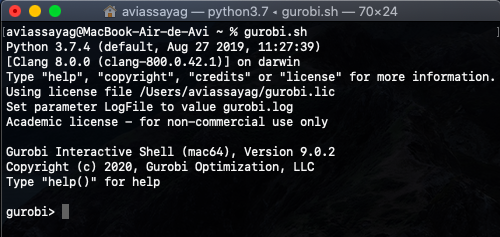
\includegraphics[scale=0.8]{console.png}
\caption{Shell interactive Gurobi }
\end{figure}
\end{center}

\subsubsection{Exemple de programmation linéaire avec Gurobi}
Soit x1 et x2 les quantités (en volume) respectives produite pour les bières b1 et b2. Les quantités sont soumises à des contraintes (3) pour chaque ingrédients utilisé : \newline \textsf{Contraintes : }
\begin{itemize} 
\item   Contrainte C1 : 2,5 x1 + 7,5 x2  $\leq$ 240 (pour le maïs)
\item   Contrainte C2 : 0,125 x1 + 0,125 x2 $\leq$ 5 (pour le houblon)
\item   Contrainte C3 : 17,5 x1 + 10 x2  $\leq$ 595 (pour le malt)
\item  Contrainte  de positivité : x1 , x2 > 0
\end{itemize}
\textsf{Objectif : }
\begin{itemize} 
\item Maximiser : max 15 x1 + 25 x2
\end{itemize}

\begin{verbatim}
#Appel et utilisation de Gurobi et de ses modules
import gurobipy as gp
from gurobipy import *


try : 
    # Création du model
    m = gp.Model("Biere")


    # Déclaration des Variables
    x1 = m.addVar(vtype=GRB.INTEGER, name="x1")
    x2 = m.addVar(vtype=GRB.INTEGER, name="x2")
   
   
   # Maximisation
    m.setObjective(15*x1 + 25*x2, GRB.MAXIMIZE)
    

    # Contraintes des Variables
    m.addConstr(2.5 * x1 + 7.5 * x2 <= 240, "c1")
    m.addConstr(0.125 * x1 + 0.125 * x2 <= 5, "c2")
    m.addConstr(17.5 * x1 + 10 * x2 <= 595, "c3")
    
   
    # Résoud la solution objective 
    m.optimize()

     #Affichage de la réponse
    for v in m.getVars():
        print('%s %d' % (v.varName, v.x))

    print('Obj: %s' % m.objVal)

     #Vérification des exceptions
except gp.GurobiError as e:
    print('Error code ' + str(e.errno) + ': ' + str(e))

except AttributeError:
    print('Encountered an attribute error')    
\end{verbatim}
\paragraph*{}{Ci dessus le code python utilisé pour permettre a \textsf{Gurobi} de trouver la solution de maximisation, soit  : \textbf{x1= 12 et x2 = 28}}
\newpage







\section{Théorie des jeux}

\subsection{Jeux statiques}
\subsubsection{Principes et modèles des jeux statiques }
\paragraph{Principe des jeux statiques}
Comme nous l'avons expliqué un peu plus haut, l'un des objectifs de ce stage est la modélisation d'algorithmes afin de résoudre des jeux stochastiques. Mais tout d'abord détaillons un peu le concept des \textsf{jeux}. \newline

Pour intégrer et comprendre ce concept, il y a d'autres notions à connaitre telles que \textsf{jeux statiques} , \textsf{jeux dynamiques} , \textsf{stratégie}, \textsf{concurrent}  ou encore \textsf{jeux bimatricel} et enfin \textsf{gain}.\newline

Comme vous l'avez compris,un jeu nécessite la présence d'acteurs ; dans la suite de nos explications lorsque nous parlerons de \textsf{joueurs} nous ferons donc référence aux acteurs du jeu.

\paragraph{Modèle des jeux statiques}
\begin{definition}
Un jeu est dit statique lorsque le jeu se déroule en une seule étape et de manière simultanée sans avoir accès aux informations de l'actions de ou des autres joueurs.
\end{definition} 

Ainsi un \textsf{jeu statique} peut être défini par : 
\begin{itemize}
\item Un nombre fini J de joueurs : {1,2, ....., J}
\item Pour chaque joueur \textsf{i}, un ensemble de stratégies $ \Pi^{i} $ = \{ $ \pi^{1} ,...,\pi{j} $\}
\item Pour chaque joueur \textsf{i} une fonction de valeur \textsf{v}$_{i}$ tel que : 
$ \Pi^{i} \times ... \times \Pi^{j} \rightarrow \mathbf{R} $
\end{itemize}

\begin{definition}
On appelle stratégie la manière dont un joueur choisit l'action qu'il effectue. C'est un vecteur de taille |A$ _{i} ^{1}$| où |A$ _{i} ^{1}$| est l'ensemble des actions du joueur A,, |A$_{i}$| est le cardinal de l'ensemble A'. Ce vecteur est noté $\pi^{1}$ pour le joueur 1 et $\pi^{2}$ pour le joueur 2.
\end{definition}

Lorsque l'on parle de stratégie pure il s'agit d'une stratégie déterministe c'est à dire une stratégie dans laquelle une seule et unique action est effectuée. Elle détermine en particulier l'action qu'un acteur (joueur) réalisera devant toutes les situations auxquels ce dernier sera confronté. \newline

\begin{definition}
On note par $ \pi^{1}(i)$ la cordonné d'indice i du vecteur $\pi^{1}$ représentant le choix d'un joueur, ce choix est déterministe. Par convention :   $\pi^{1}(i) = 0$ l'action n'est pas choisie et  $\pi^{1}(i) =1$ l'action est choisie.
\end{definition}

En parallèle aux stratégies pures, il existe aussi des stratégies dites mixtes c'est à dire ou chaque action d'un joueur i  dépend d'une probabilité (connue ou non) provenant de la stratégie pure du même joueur. \newline


\begin{definition}
L'action est choisie en fonction d'une probabilité. Le vecteur $\pi^{1}$ est maintenant une distribution  de probabilité sur les actions du joueur. $\pi^{1}(i)$ est la probabilité que l'action i soit choisie. De plus comme  $\pi^{1}$ est une probabilité on à obligatoirement $\underset{i}{\Sigma}  \hspace{0,2 cm} \pi^{1}(i) = 1$.
\end{definition}

\paragraph{Equilibre de Nash}
{Maintenant que l'on en connait un peu plus sur le concept fondamental de la \textsf{théorie des jeux} nous avons bien compris que résoudre un jeu (dynamique bien évidement) revient non pas à "gagner" la partie mais trouver la meilleur stratégie permettant de maximiser ses gains et donc a fortiori minimiser ses pertes (puisqu'elles correspondent à gain réciproque des autres acteurs).} 

\begin{definition}
Une action conjointe a* est un équilibre de Nash si et seulement si : $ \forall $j, $ \forall a_{j}$ R$ _{j} $(a*) $ \geq $ R$ _{j} $(a$ _{j} $,a*$ _{-j} $).
\end{definition}


\subparagraph*{}{Autrement dit, trouver \textsf{un équilibre de Nash} dans un jeu revient a trouvé la solution optimal de stratégies mixtes (x,y) qui sont meilleurs réponses l'une fonction de l'autre, c'est à dire :}
\begin{itemize}
\item x est la meilleur réponse dans la stratégie de y (J2) qui maximise la matrice de gain du J1 donc x.
\item y est la meilleur réponse dans la stratégie de x (J1) qui maximise la matrice de gain du J1  donc x
\end{itemize}  


\subparagraph{Nash en stratégie pure}{Un profil de stratégie est un ensemble de spécifiant pleinement pour tout joueur, toutes les actions dans le jeu. Il comporte une et une seule stratégie pour chaque joueur.}
\begin{definition}
Soit $\pi^{i} $ une stratégie du joueur i et $ \pi^{-i} $ la stratégie des autres joueurs. Un profil de stratégies $\pi^{*} = \pi^{i}$ est un équilibre de Nash si et seulement si :
\end{definition}
\begin{align*}
\forall i, \hspace{0,2 cm} \forall \pi^{'i} \hspace{0,2 cm} \in \hspace{0,2 cm} \Pi^{i}, \hspace{0,2 cm} v_{i}(\pi^{i}\hspace{0,1 cm}, \pi^{-i}) \hspace{0,2 cm} \geq \hspace{0,2 cm} v_{i}(\pi^{'i}\hspace{0,1 cm}, \pi^{-i})
\end{align*}

\subparagraph{Nash en stratégie mixte}{On appelle $\sigma^{i}$  une stratégie mixte (ou profil de stratégie mixte) une distribution de probabilités sur les actions. L’ensemble des stratégies mixtes du joueur i est noté S$^{i}$.}
\begin{definition}
Soit $\sigma ^{*} $ un profil de stratégie mixte. $\sigma ^{*} $est un équilibre de Nash si, pour tout joueur i on a : 
\end{definition}
\begin{align*}
\forall \sigma ^{'i}, \hspace{0,2 cm} \in \hspace{0,2 cm} S^{i}, \hspace{0,2 cm} v_{i}(\sigma ^{*i} , \hspace{0,1 cm} \sigma^{*-i}) \hspace{0,2 cm} \geq (\sigma ^{'i} , \hspace{0,1 cm} \sigma^{*-i})
\end{align*}


\subsubsection{Jeux bimatrciel}
Un jeu bimatriciel se caractérise comme son nom l'indique par deux matrices. Ces dernières ne sont autres que les gains des joueurs. Autrement dit les joueurs jouent de manière simultané et on inscrit dans une matrice leurs gains (une matrice pour chaque joueur). Pour la suite du mémoire et du stage nous allosn donc utiliser strictement des jeux à deux joueurs JA et JB.

Ainsi un \textsf{jeu bimatriciel} est défini par :
\begin{itemize}
\item Un nombre fini J de joueurs : \{1,2, ....., J\}
\item Un nombre fini M d'actions pour le joueur 1 (JA) :\{1,2, ....., M\}
\item Un nombre fini N d'actions pour le joueur 2 (JB) : \{1,2, ....., N\}
\item Une matrice de gain (pay-off) G1 pour le joueur JA  [M $\times$ N]
\item Une matrice de gain (pay-off) G2 pour le joueur JB  [N $\times$ M]
\item Une stratégie pure par joueurs composé des actions des joueurs respectifs
\end{itemize}

\paragraph{Exemple de jeu bimatriciel}
\[
Joueur\hspace{0,1cm} A\hspace{1cm}
\begin{pmatrix}3&3\\
2&5\\
0&6\\
\end{pmatrix}\                      \hspace{2,5cm}  
Joueur\hspace{0,1cm} B \hspace{1cm}  
\begin{pmatrix}3&2\\
2&6\\
3&1\\
\end{pmatrix} 
\]

\paragraph{Équilibre en stratégie pure}
D'après les matrices précédentes  le seul équilibre pur (obtenu par le théorème du \textsf{minimax}) est  \textbf{x = \{(1,0,0) , (1,0)\}}.
\subparagraph*{}{Pour vérfiier cela il semble logique que si JA choisi (1,0,0) \textsf{soit 3} et JB choisi (1,0) \textsf{soit  3} il apparait un équilibre pur puisque le gain de JA serait de 3 et JB 3 aussi. C'est bien la seule solution possible pour équilibre.

\paragraph{Équilibre en stratégie mixte}
On cherche a savoir si il existe un support de la forme x=($x_{1},x_{2},0$) et y=($y_{1}, y_{2}$) correspondant à une stratégie mixte tel que ($x_{1},x_{2},y_{1}, y_{2} > 0$). 

insi d'après les donnés précédentes, x = (x$_{1}$, x$_{2}$) et y = (y$_{1}$, y$_{2}$) impliquent respectivement que (Ay$ _{1} $) et (Ay$ _{2} $) ont la même valeur tout comme (Bx$ _{1} $) et (Bx$ _{2} $). D'ou le système suivant : }
\begin{align*}
\left \{
   \begin{array}{r c l}
      3x_{1} + 2x_{2} & = & \textsf{v} \\
      2x_{1} +6x_{2}  & = &\textsf{v}  \\
      x_{1} + x_{2} & = & 1
   \end{array}
   \right.
   & \hspace{3 cm}
   \left \{
   \begin{array}{r c l}
     3y_{1} + 3y_{2} & = & \textsf{w} \\
     2y_{1} + 5y_{2}  & = &\textsf{w}  \\
      y_{1} + y_{2} & = & 1
   \end{array}
   \right .
\end{align*}
ce qui nous donne : 
\begin{align*}
\left \{
   \begin{array}{r c l}
      x_{1}  & = & 4x_{2} \\
      x_{1} + x_{2} & = & 1 
   \end{array}
   \right.
   & \hspace{3 cm}
   \left \{
   \begin{array}{r c l}
     y_{1} & = & 2y_{2}  \\
      y_{1} + y_{2} & = & 1  
   \end{array}
   \right .
\end{align*}
\subparagraph{}{Ainsi il apparait rapidement les stratégies mixtes suivantes : 
\begin{align*}
     x=(\frac{4}{5}, \frac{1}{5},0)
   & \hspace{3 cm}
  y=(\frac{2}{3}, \frac{1}{3}).
  \intertext {donnant les vecteur de PayOff respectif :}
      Ay=(3,3,2)
   & \hspace{3 cm}
  Bx=(\frac{14}{5}, \frac{14}{5}).
  \intertext {pour un PayOff total respectif :}
   x^{t}Ay=(3)
   & \hspace{3 cm}
  x^{t}By=(\frac{14}{5}).
\end{align*}

\subsubsection{Jeux à somme nulle}
Comme annoncé dans notre introduction nous essayerons de résoudre des jeux à sommes nulles via des algorithmes que nous allons implémenter par la suite. Mais qu'est ce qu'un jeu à somme nul ? \newline

Un jeu à somme nul est un jeu où le gain d'un des acteurs (J1, par exemple) représente la perte équivalente réciproque des autres acteurs ((J2, par exemple). Pour faciliter la compréhension et la résolution de ces modèles, le nombre d'acteurs autrement dit de joueurs sera fixé à 2.\newline


\subparagraph*{}{Il existe plusieurs jeux ou situations "connus" que l'on pourrait assimiler à un \textsf{jeu à somme nulle} comme le jeu de \textsf{pile ou face} mais nous allons nous plonger sur un autre jeu un peu moins connu \textsf{Matching pennies} et nous allons essayer de mieux comprendre qu'est ce qu'un \textsf{jeu a somme nulle} et surtout comment le gagner ou du moins trouver la meilleur solution.}

\subsubsection{Un exemple de jeu :  "Matching pennies"}
Si l'on essaie de traduire mot - a - mot le nom du jeu on obtient : "jeux d'appariement de sous"  ; évidemment cela ne nous avance pas plus. Alors comment pourrions nous définir et mieux intégrer le jeu \textsf{matching pennies} ? \newline

C'est un jeu simple et l'un plus connu dans le concept de la théorie des jeux, il se joue seulement à deux joueurs JA : \textsf{Pair}  et JB : \textsf{Impair}. Chaque acteurs (Pair \& Impair) possèdent une pièce et choisissent simultanément et secrètement une des deux faces \textsf{Pile} ou \textsf{Face}, puis en fonction des résultats obtenu on assiste des scénarios de gains différents :

\begin{itemize}
\item Les deux faces des pièces correspondent et dans ce cas Pair garde les deux pièces (+1 Pair, -1 Impair)
\item Les deux faces des pièces ne correspondent pas et dans ce cas Impair garde les deux pièces (+1 Impair, -1 Pair)
\end{itemize}  \vspace{0.2 cm}

\begin{figure}[h!]
\centering
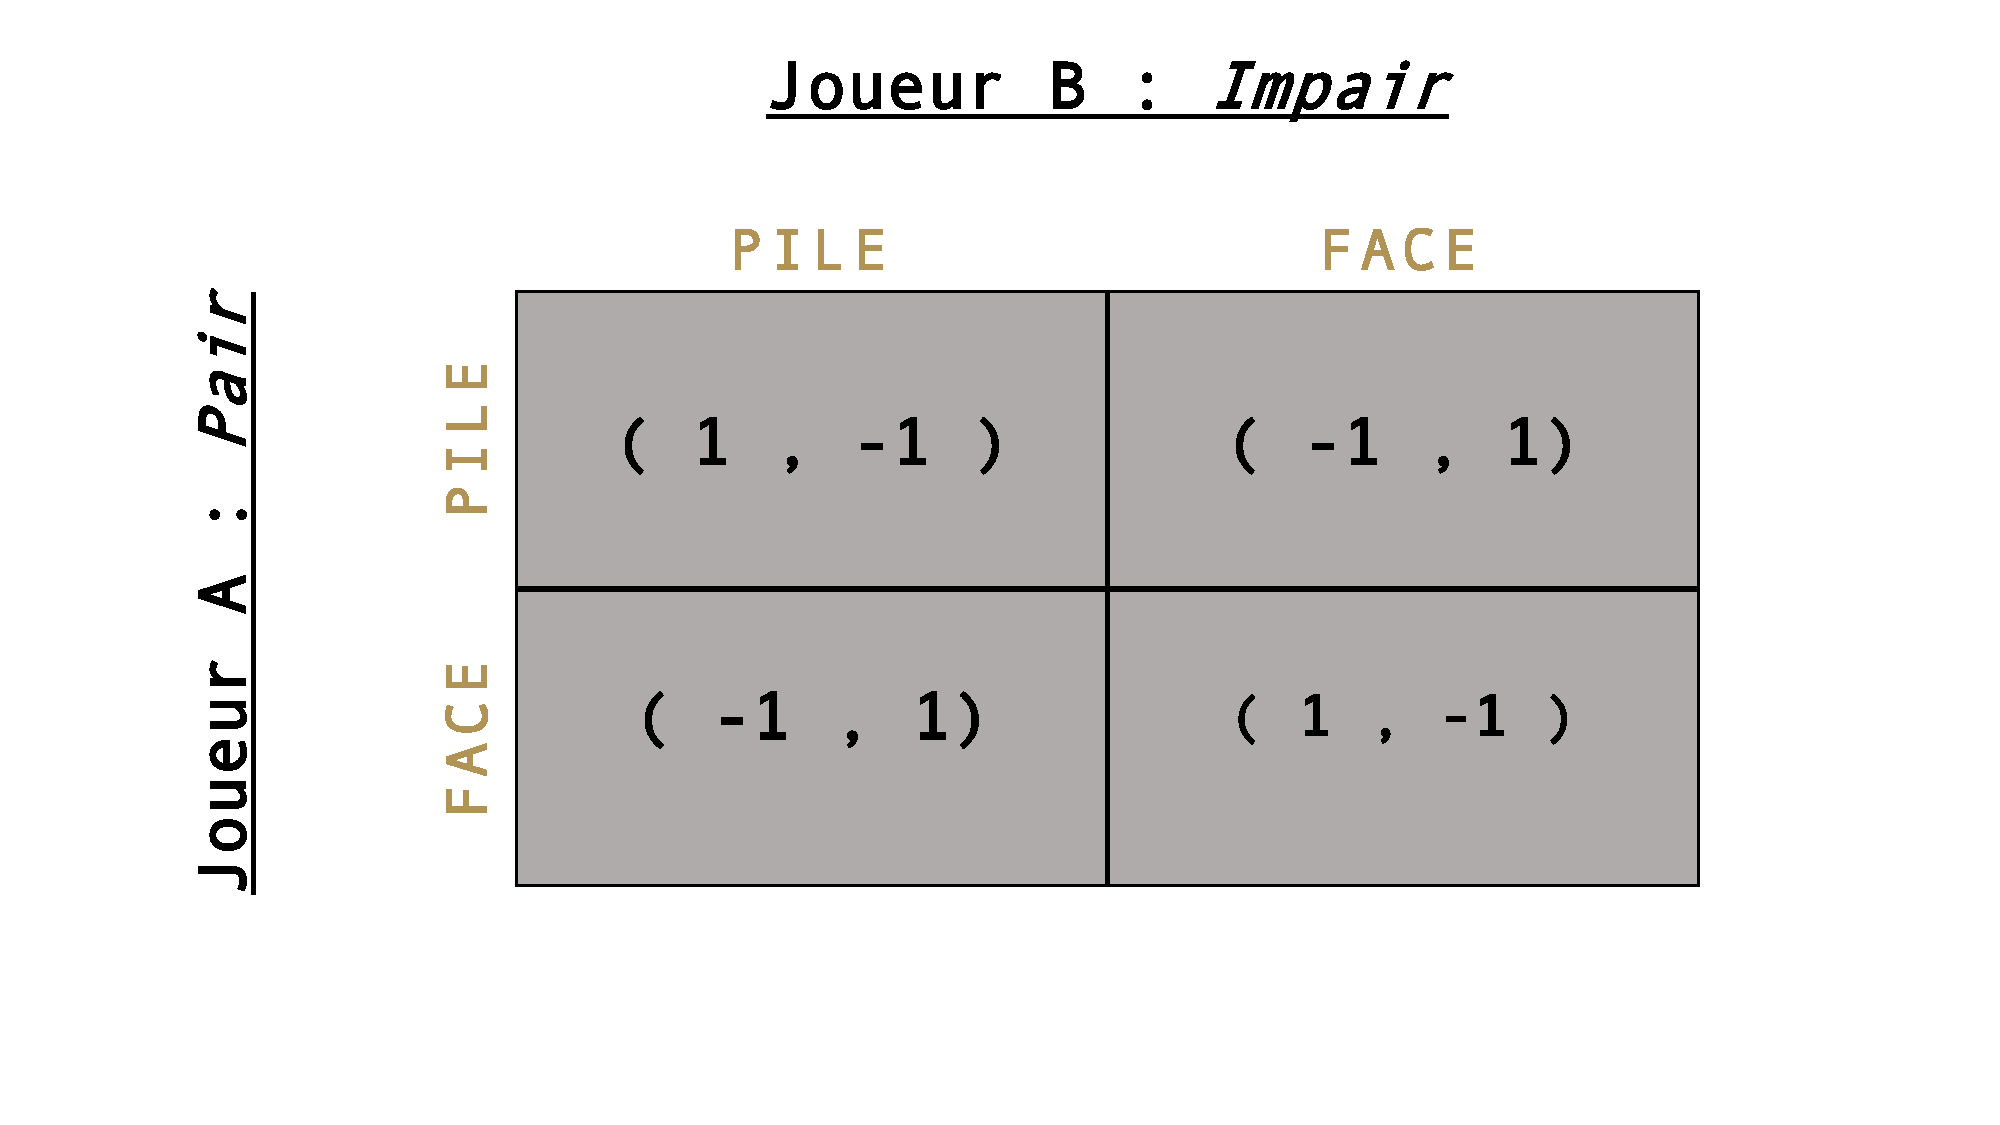
\includegraphics[scale=0.4]{Matching.pdf}
\caption{Represenation matricielle de "Matching Pennies"}
\end{figure} 

\subparagraph*{}{Ainsi d'après ce que nous avons déjà vu dans les sections précédentes on peut comprendre que \textsf{matching pennies} est un jeu à somme nulle puisque le gain d'un des deux joueurs (par exemple Pair) est bien la perte réciproque de l'autre joueur (ici Impair).} 
\subparagraph*{}{De même vous aurez compris que ce jeu permet aussi d'illustrer le concept  de stratégies et de l'\textsf{équilibre de Nash} cependant cette configuration n'admet pas de stratégie pure pour l'\textsf{équilibre de Nash} mais plutôt une stratégie mixte reposant sur le choix probabiliste de chaque joueurs à choisir une des deux faces de la pièce.}

\subparagraph*{}{Puisque c'est un jeu bi-matricel a somme nulle, profitons de sa définition même pour avoir une vue d'ensemble sur le jeu ; c'est à dire les actions de chaque joueurs mais aussi les gains ou pertes respectifs en fonction des choix effectués (cf [4.1.1]).} \newline

Pour la représentation du jeu nous allons estimer que le gain ou perte est de de 1 puisque c'est avec une seule pièce que nous jouons, que le joueur JA \textsf{Pair} joue sur les lignes tandis que le joueur JB \textsf{Impair} joue les colones.  \vspace{0.4 cm}

\paragraph{Matrice de gains des joueurs A et B}{Ainsi comme nous l'expliquons depuis plusieurs paragraphes, le propre même du jeu bimatricel repose sur l'existence de la matrice de "gain" ou de "payoff".  Nous allons donc donner la matrice de gain A de JA \textsf{Pair} et celle de JB \textsf{Impair} qui n'est autre que l'opposé de celle de  A (B = - A).}

\[
Matrice\hspace{0,1cm} A\hspace{1cm}
\begin{pmatrix}1&-1\\
-1&1\\
\end{pmatrix}\                      \hspace{2,5cm}  
Matrice\hspace{0,1cm} B \hspace{1cm}  
\begin{pmatrix}-1&1\\
1&-1\\
\end{pmatrix} 
\]

\subsection{Jeux bimatriciel a sommes nulles et résolution par PL}
%Blablate sur le jeux

C'est alors qu'intervient la notion de \textsf{stratégie} (ou encore, règles de décision) pour  qu'un acteur puisse prendre une décision affin d'effectuer une future action dans le jeu.\newline
\begin{definition}
La stratégie d’un acteur est l’une des options qu’il choisit dans un contexte où son choix dépend non seulement de ses propres actions, mais également de celles des autres.
\end{definition}

On peut donc distinguer deux grandes catégories de \textsf{stratégies} soit pures soit mixtes, nous rentrerons en détails dans les sections suivantes (respectivement [4.2.1] et [4.2.2]. \newline

Maintenant que nous avons abordez la notion de stratégie, intéressons nous à la programmation linéaire. La "victoire" ou "réussite" d'un jeu se traduit mathématiquement par le \textsf{gain} le plus élevé. Ainsi le but est donc de d'utiliser la stratégie la plus optimale qui permettrait de maximiser les \textsf{gains} du jeu.

\begin{definition}
La programmation linéaire (PL) est un problème d'optimisation où la fonction objectif et les contraintes sont toutes linéaires. Le but de résoudre un PL est de trouvé les variables optimales qui maximisent la fonction objective.
\end{definition}

C'est donc grâce à la \textsf{programmation linéaire} (via une implémentation sur \textsf{Gurobi}) que nous arriverons a trouvé la solution optimal et dans le meilleur des cas \textsf{l'équilibre de Nash}[4.2.3]. \newline

D'une approche plus mathématiques on peut résumer la résolution d'un \textsf{jeu statique} par \textsf{programmation linéaire} comme ceci : \newline
\begin{align*}
\large \textsf{max} \hspace{0,2 cm} \textsf{min} \hspace{0,2 cm} \sum_{i=0}\hspace{0,2 cm} \pi_{i}^{1}\hspace{0,2 cm} a _{ij}  =\hspace{0,2 cm} \textsf{max} \hspace{0,2 cm} \textsf{min} \hspace{0,2 cm}\Sigma _{i}\hspace{0,2 cm} \Sigma _{j}\hspace{0,2 cm} \pi_{i}^{1}\hspace{0,2 cm} a _{ij} \hspace{0,2 cm} \pi_{j}^{2} 
\end{align*}

Expliquons un peu plus cette formule; $ \pi $ est un probabilité relative à une stratégie donc 
$\pi_{i}^{1}$ est la stratégie relative 1 en fonction de i (etc...), quand à a$ _{ij} $ il s'agit de la matrice (ligne \textsf{i} x colonne \textsf{j}) de gain ou récompense de A (donc du premier joueur).  Le but même est de trouver, pour A, la stratégie mixte répondant à l'objectif de maximiser les gains de A. \newline

Ainsi le joueur A, doit résoudre :
\begin{align*}
\large {\textsf{max} \hspace{0.2 cm} \textsf{min} \hspace{0.2 cm} \Sigma_{i}\hspace{0.2 cm} \pi_{i}^{1}\hspace{0.2 cm} a _{ij} } \\ s.c \hspace{0,4 cm}
\large {\Sigma_{i}\hspace{0,2 cm}\pi_{i}^{1} = \hspace{0,2 cm}1}
\end{align*}
\paragraph*{}{Puisque $\pi_{i}^{1}$ étant une probabilité, sa somme ne peut pas être supérieur a 1. Cependant nous ne somme pas en présence encore d'un programme linéaire (dont nous avons connaissance de technique de résolution), pour cela nous allons le transformer  en posant une fonction  \textsf{v} à maximiser et ceux pour chacune des sommes dont on cherche le minimum de gain (du joueur adverse , ici B)}. \newline 

Le problème devient donc sous forme linéaire (PL) avec pour fonction objective \textsf{v} à maximiser avec pour seules contraintes : 
\begin{align*}
\large{v \hspace{0.2 cm} \leq  \hspace{0.2 cm}\Sigma_{i}\hspace{0.2 cm} \pi_{i}^{1}\hspace{0.2 cm} a _{ij}} \\ et \hspace{0,2 cm} toujours : \hspace{0,4 cm}
\large{\Sigma_{i} \hspace{0.2 cm} \pi_{i}^{1} = 1}
\end{align*}
{Comme nous l'avons expliquer plus haut dans un jeu à somme nul trouver l'\textit{équilibre de Nash} n'est pas forcement possible il faut donc résonner autrement et utiliser le théoreme du \textsf{minimax}. Pour résoudre cela, il faut tenter de maximiser la stratégie pure de JA \textsf{Pair} et donc trouver : \newline
\begin{align*}
 \large {\textsf{maximiser} \underset{1 \leq j \leq m}{\textsf{min}} \hspace{0,2cm}  \underset{i}{\Sigma} \hspace{0,2cm} \pi_{i}^{1} \hspace{0,2cm}  a _{ij} }  
\end{align*}
\subparagraph*{}{Cependant le problème n'est pas tout à fait encore sous forme linéaire et donc cela il suffit de trouver la fonction à maximiser \textsf{v} tel que \textsf{v} soit plus petite que toutes les sommes que nous cherchons à minimiser. D'ou :} 
\begin{align*}
\large {\textsf{maximiser} \hspace{0,2 cm} v }\\ 
\large{ s.c \hspace{0.4 cm} v \hspace{0,2 cm} \leq  \hspace{0.2 cm}\Sigma_{i}\hspace{0.2 cm} \pi_{i}^{1}\hspace{0.2 cm} a _{ij}} \\
\large{\Sigma_{i} \hspace{0.2 cm} \pi_{i}^{1} = 1} \\ 
\large{ \pi_{i}^{1} \hspace{0,2 cm} \geq \hspace{0,2 cm} 0 \hspace{0,2 cm} \forall i }
\end{align*}




\subsubsection{Matrice de gains des joueurs A et B}{Ainsi comme nous l'expliquons depuis plusieurs paragraphes, le propre même du jeu bimatricel repose sur l'existence de la matrice de "gain" ou de "payoff".  Nous allons donc donner la matrice de gain A de JA \textsf{Pair} et celle de JB \textsf{Impair} qui n'est autre que l'opposé de celle de  A (B = - A).}

\[
Matrice\hspace{0,1cm} A\hspace{1cm}
\begin{pmatrix}1&-1\\
-1&1\\
\end{pmatrix}\                      \hspace{2,5cm}  
Matrice\hspace{0,1cm} B \hspace{1cm}  
\begin{pmatrix}-1&1\\
1&-1\\
\end{pmatrix} 
\]

 

\subsubsection{L''équilibre de Nash dans Matching Pennies}{Supposons maintenant que le JA \textsf{Pair} joue \textsf{Pile} avec une probabilité \textsf{p} (donc il joue \textsf{Face} avec une probabilité de \textsf{(1-p)} et que le JB \textsf{Impair} joue \textsf{Pile} avec une probabilité \textsf{q} (donc il joue \textsf{Face} avec une probabilité de \textsf{(1-q)} le jeu se \\
 donc sous cette forme : } 

\[
\begin{pmatrix}(pq)& p(q-1)\\
q(p-1)&(1-p)(1-q)\\
\end{pmatrix}\            
\]
\subparagraph*{}{En utilisant le théorème du \textsf{minimax} on arrive à la proposition suivante (pour JA \textsf{Pair}) : }
\begin{align*}
\begin{array}{r c l}
     pq + (1-p)(1-q) -p(1-q) -q(1-p)  & = & 4pq -2p -2q +1  \\
     & = & (1-2p)(1-2q) 
   \end{array}     
\end{align*}

\subparagraph*{}{On peut tout de suite voir que pour chaque "membre" soit positif autrement dit que JA \textsf{Pair} maximise ses gains et minimise sa perte (ou inversement avec JB \textsf{Impair} la seule situation stable s'apparente que si : 
\textbf{p = $\frac{1}{2}$} et que \textbf{q = $\frac{1}{2}$}.}


\subsection{Jeux Stochastiques}
\subsubsection{Jeux dynamqiue}
\begin{definition}
Un jeu est dynamique lorsqu'il se déroule en plusieurs étapes non simultané, c'est a dire que les joueurs jouent plusieurs fois mais en ayant connaissance des actions des autres joueurs et donc peuvent établir des stratégies.
\end{definition}

Prenons pour hypothèse un jeu dynamique à deux  J1 et J2, les deux joueurs vont effectuer tours à tours des actions en différé en ayant accès aux informations des actions du joueur précédent. \newline

Ainsi un \textsf{jeu dynamique} peut être défini par : 
\begin{itemize}
\item Un nombre fini J de joueurs : \{1,2, ....., J\}
\item Un nombre identique d'actions K par joueurs : \{1,2,....K\}  
\item Un ensemble infini E d'états du jeu qui sont indicé par les actions des joueurs 
\item Une stratégie pure par joueurs composé des actions des joueurs respectifs
\end{itemize}

\subsubsection{Fonction de valeur}
Le critère d'évaluation d'une stratégie $\pi$ correspond à l'espérance mathématique de la somme des gains obtenus en suivant cette stratégie et en partant d’un sommet initial \textsf{s},  cette espérance est appelée \textsf{fonction de valeur}.

\subparagraph*{}{Rappelons le tout de même une stratégie $\pi_{i}(s)$ dépend de l'action choisi par le joueur \textsf{i} à l'état \textsf{s} en stratégie pure et $\pi_{i}(s,a)$ en stratégie mixte avec une probabilité \textsf{a} pour l'état \textsf{s}}.

\subparagraph*{}{L'une des variantes les plus connues est de pondérer les gains par un facteur $\gamma \in $ [0;1[ afin de prendre en compte la valeur des gains futur. En notant r$_{t}$ la récompense reçue à l'instant \textsf{t} $ \in $ K et \textsf{s$^{0}$} l'état initial, on définit la \textsf{fonction de valeur} pour tout \textsf{s} $\in $ S pour une stratégie $ \pi$ :}
\begin{align*}
V^{\pi}(s) \hspace{0,1 cm} = \hspace{0,1 cm} E^{\pi}\hspace{0,1 cm} (\sum_{t=0}^{\infty} \hspace{0,1cm}\gamma ^{t} \hspace{0,1cm} r^{t}\hspace{0,1cm} |\hspace{0,1cm} s^{0} = s )
\end{align*}


\subsubsection{Modèles et principes de jeux stochastiques }
Au début de chaque étape, le jeu est dans un certain état . Les joueurs sélectionnent des actions et chaque joueur reçoit un gain cela dépend de l'état actuel et des actions choisies. Le jeu passe alors à un nouvel état aléatoire dont la distribution dépend de l'état précédent et des actions choisies par les joueurs. La procédure est répétée au nouvel état et le jeu continue pour un nombre fini ou infini d'étapes. Le gain total pour un joueur est souvent considéré comme la somme actualisée des gains de l'étape ou la limite inférieure des moyennes des gains de l'étape.

\paragraph{Modèles des jeux stochastiques}
On définit $\Phi$ un jeu stochastique fini à somme nulle tel que :
\begin{itemize}
\item Un ensemble $\Omega$ fini d'états
\item I l'ensemble fini d'action du joueur A
\item J l'ensemble fini d'action du joueur B
\item Une fonction de paiement $g : I \times J \times\Omega\rightarrow [ -M,M]$ (max JA et min JB)
\item Une probabilité de transition d'état $\rho : I \times J \times \Omega \rightarrow \Delta (\Omega)$
\end{itemize}

\paragraph{Principes des jeux stochastiques}
On part d'un état $\omega_{1}$ donné et connu des deux joueurs (JA et JB), pour chaque étape $t \in \mathbf{N}$ on observe :
\begin{itemize}
\item JA et JB observe $\omega_{t}$ l'état courant et se rappelle des états précédents
\item Simultanément et respectivement JA choisit une action mixte $x_{t}$ dans $X = \Delta (I)$ et JB choisit une action mixte $y_{t}$ dans $Y = \Delta (J)$ 
\item Respectivement JA effectue une une action $i_{t} $ en fonction de $x_{t}$ et JB effectue une une action $j_{t} $ en fonction de $y_{t}$
\item Une étape de paiement $t : g_{t} = g\hspace{0,1 cm} (i_{t},j_{t},\omega_{t})$ 
\item L'état suivant $\omega_{t+1}$ attribué selon $\rho \hspace{0,1 cm} (i_{t},j_{t},\omega_{t})$ 
\end{itemize}
\subparagraph*{}{Ainsi, dans un jeu stochastique, chaque action conjointe mène tous les joueurs à un nouvel état où se jouel ’équivalent d’un jeu statique avec des gains particuliers à chaque état. En théorie, dans un jeu stochastique, les probabilités de transition peuvent dépendre de l’historique de tous les états passés ; lorsque les probabilités de transition ne dépendent que de l’état courant, il s’agit au sens strict d’un jeu de Markov. Durant le stage, on considérera uniquement des jeux où les probabilités de transition ne dépendent que de l’état courant.}

\subparagraph*{}{À la différence des jeux statiques, les jeux stochastiques ne disposent pas de solutions optimales qui soient indépendantes des joueurs. Par conséquent, il faut définir la notion de stratégie optimale de manière analogue à
celle d’un jeu classique. Ainsi, en notant $\Pi_{j}$ l’ensemble des stratégies possibles du joueur $j$, on peut adapter la notion\textsf{d’équilibre de Nash} aux jeux stochastiques.

\paragraph{Équilibre de Nash en jeux stochastiques}
\begin{definition}
Une stratégie conjointe $\pi^{*}$ est un équilibre de Nash si et seulement si : 
\end{definition}
\begin{align*}
\forall s \in S,\hspace{0,2 cm} \forall j \in J, \hspace{0,2 cm} \forall \pi_{j} \in \Pi_{j}, \hspace{0,2 cm} V_{j}^{\pi*}(s) \hspace{0,2 cm}\geq \hspace{0,2 cm} V_{j}^{\pi_{j},\pi_{-j}^{*}}(s)
\end{align*}
\newpage
\section{Conclusions}
\subsection{Contributions apportées}
\subsection{Difficultés rencontrées}
\subsection{Axes d'amélioration}

\newpage
\section{Webographie}
\begin{thebibliography}{2}
 \bibitem[Paris X (Nanterre)]{Paris X}\url{https://www.parisnanterre.fr/}\newline 
   \bibitem[GitHub]{GitHub}\url{https://help.github.com/en}\newline
   \bibitem[Python]{Python} \url{https://docs.python.org/fr}\newline
   \bibitem[Gurobi]{Gurobi}\url{ https://www.gurobi.com/downloads/gurobi-software/}\newline
   \bibitem[Gurobi]{Gurobi}\url{ https://www.gurobi.com/documentation/9.0/refman/py_model.html}\newline
   \bibitem[Théorie des Jeux]{RO}\url{https://fr.wikipedia.org/wiki/Th\%C3\%A9orie_des_jeux}\newline
   \bibitem[Théorie des Jeux]{RO}\url{http://www.cril.univ-artois.fr/~konieczny/enseignement/TheorieDesJeux.pdf}\newline
   \bibitem[Théorie des Jeux]{RO}\url{http://www.cril.univ-artois.fr/~konieczny/enseignement/TheorieDesJeux.pdf}\newline 
   
\end{thebibliography}

\newpage
\section{Annexes}
\subsection{Nanterre}
\begin{center}
\begin{figure}[h!]
\centering
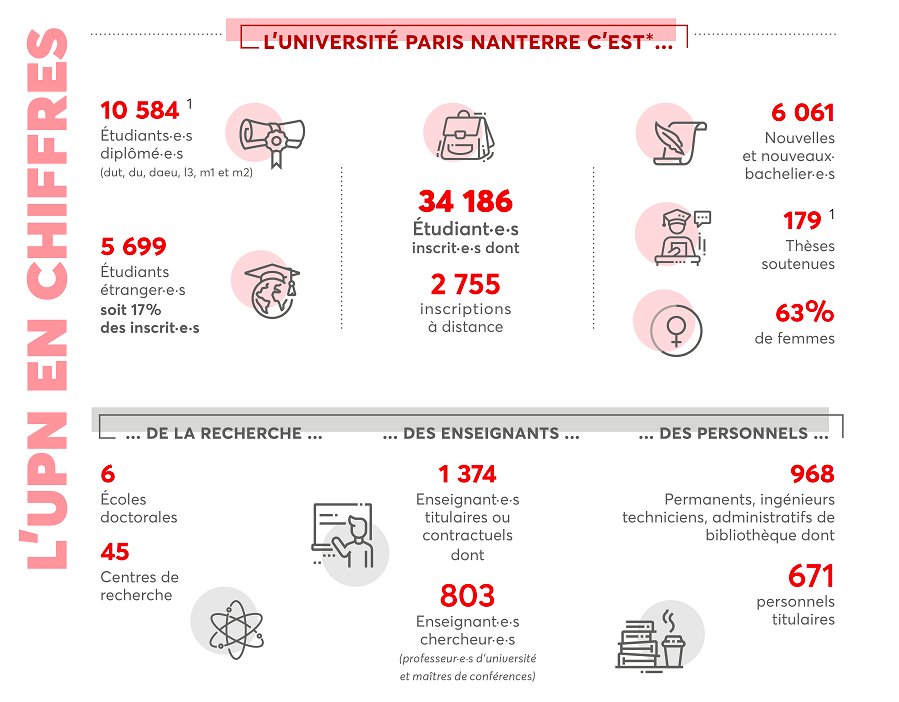
\includegraphics[scale=0.4]{chiffres.png}
\caption{L'Université Paris X en chiffres}
\end{figure}
\end{center}

\begin{center}
\begin{figure}[h!]
\centering
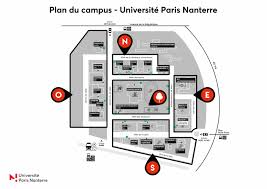
\includegraphics[scale=1.3]{plan.jpeg}
\caption{Le plan de Paris X}
\end{figure}
\end{center}
\subsection{Python en général}
La syntaxe est assez similaire aux autre langage puisque python utilise les mêmes types de variables, sauf les types sophistiqués. A la différence des autres langages de programmation (C,,C++,Java,php) la fin d'une instruction se termine par un caractère vide
et non  ; , avec python c'est l'indentation qui fait office d'instruction et donc de bloc de code.
\subsubsection{ Structure Conditionelle If }
La condition est suivi par  :  puis vient ensuite l'instruction à effectuer, si le test est vérifié, qu'il faudra indenter (d'un cran).
\begin{verbatim}
if <condition> :
      <instruction>
\end{verbatim}
\subsubsection{ Structure Conditionelle Else}
La condition est suivi par  :  puis vient ensuite l'instruction à effectuer, si le premier test n'est pas vérifié, qu'il faudra indenter (d'un cran) au même niveau que le test If.
\begin{verbatim}
if <condition1> :
      <instruction1>
else :
      <instruction2>
\end{verbatim}
\subsubsection{ Structure Conditionelle Elif }
La condition est suivi par  :  puis vient ensuite l'instruction à effectuer, si le premier test n'est pas vérifié, qu'il faudra indenter (d'un cran) au même niveau que le test If.
\begin{verbatim}
if <condition1> :
      <instruction1>
elif <condition2> :
      <instruction2>
else : 
      <instruction3>
\end{verbatim}
\subsubsection{ Boucle For}
La structure est composé de for puis de deux valeurs élément et sequence qui permette de suivre l'itération à effectuer. Le bloc est exécuté autant de fois de qu'il y a d' éléments dans la sequence et se termine par  : .
\begin{verbatim}
for element in sequence :
     <instruction>
\end{verbatim}
\subsubsection{ Boucle While }
La structure est composé de while puis de la condition qui permet d'effectuer un test. Le bloc est exécuté tant que la condition est vérifié et se termine par  : .
\begin{verbatim}
while <condition> :
     <instruction>
\end{verbatim}
\subsubsection{ Les fonctions}
Quant au fonction la définition se fait de manière très simple il suffit d'utiliser le mot clé def et cela est terminer, en python on ne prend pas en compte le type de retour d'une fonction comme en C, C++ ou en Java (int, void, double, float etc ...).
\begin{verbatim}
def onction (param1 , param2) :
    <instruction1>
    <instruction2>
        if <test1> :
            <instruction3>
        else :
            <instruction4>
    return  <instruction5>
\end{verbatim}

\subsection{L'orienté objet en Python}
Python est un langage résolument orienté objet, ce qui signifie que le langage tout entier est construit autour de la notion d’objets. Quasiment tous les types du langage String / Integer / Listes / Dictionnaires  sont avant tout des objets tout comme les fonctions qui elles aussi sont des objets.

\subsubsection{Création de class}{Pour créer une classe , donc un Objet il suffit d'utilise le mot clé class suivit de  :  et ne pas oublier l'indentation.}
\begin{verbatim}
class < NomClasse> : 
     attribut1
     attribut2 
\end{verbatim}

\subsubsection{Création du constructeur}{Ensuite il faudra définir un constructeur qui permettra d'instancier les objets dont nous auront besoins, il faut donc utiliser la méthode  \textsf{init} au sein de la classe sans oublier le paramètre obligatoire (mot clé de python) \textsf{self}. }

\begin{verbatim}
class < NomClasse> : 
    attribut1
    attribut2 

    def __init__ (self):
        self.attribut1 = ... (str)
        self.attribut2 =  ...  (int)
\end{verbatim}

\subsubsection{Le mot clé pass}{Si l'on défini une classe vide c'est a dire ou pour le moment il n'y aucune action à effectuer il faut rajouter le mot clé \textsf{pass}.}
\begin{verbatim}
class < NomClasse > : 
    pass 
\end{verbatim}
\subsubsection{L'héritage en python}{Comme nous l'avons également vu ont une classe mère peut hérité d'une autre et donc de ses attributs et de ses méthodes. la syntaxe est simple, il suffit de mettre en paranthése la classe mère au moment de la déclaration de la classe fille. Voici un exemple avec <NomClasse > et < NomClasse2>.}
\begin{verbatim}
class < NomClasse> :                         #classe mère
    attribut1
    attribut2 

class < NomClasse2> (< NomClasse >) :        #classe fille
    attribut1                                #hérité 
    attribut2                                #hérité 
    attribut3   
    attribut4
\end{verbatim}
\subparagraph{}{A ce niveau on peut se demander comment Python gére ces héritages. Lorsqu’on tente d’afficher le contenu d’un attribut de données ou d’appeler une méthode depuis un objet, Python va commencer par chercher si la variable ou la fonction correspondantes se trouvent dans la classe qui a créé l’objet.}

\subparagraph{}{Si c’est le cas, il va les utiliser. Si ce n’est pas le cas, il va chercher dans la classe mère de la classe de l’objet si cette classe possède une classe mère. Si il trouve ce qu’il cherche, il utilisera cette variable ou fonction.}

\subparagraph{}{Si il ne trouve pas, il cherchera dans la classe mère de la classe mère si elle existe et ainsi de suite. Deux fonctions existent pour savoir si l'objet est seulemnent  une instance d'une classe et pour savoir si la classe en question a eu recourt à de l'hériatge : isinstance() et issubclass(). }

\subsection{GitHub}
En résumé les commandes principales de \textsf{Github}.
\begin{center}
\begin{tabular}{|l|l|}
\hline
git init & git remote add \\ \hline
git clone & git checkout \\ \hline
git branch < branche > &  git branch -d < branche > \\ \hline
git add < fichier > &  git add * (pour tous les fichiers) \\ \hline
git commit -m ".." &  git merge \\ \hline
git push origin < branche > & git pull origin < master >  \\ \hline
\end{tabular}
\end{center}
\newpage
\subsection{Gurobi}
Voici les deux méthodes (via gurobi.sh ou alors via le module gurobipy) que l'on peut utiliser pour résoudre un programme MIP nommé "biere.py" (voir exmeple [5.3]) :
\begin{center}
\begin{figure}[h]
\centering
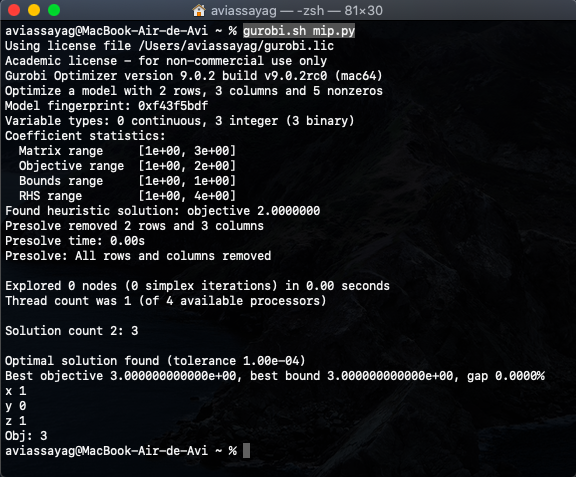
\includegraphics[scale=0.4]{gurobish.png}
\caption{Résolution via shell gurobi (gurobi.sh)}
\end{figure}
\begin{figure}[h]
\centering
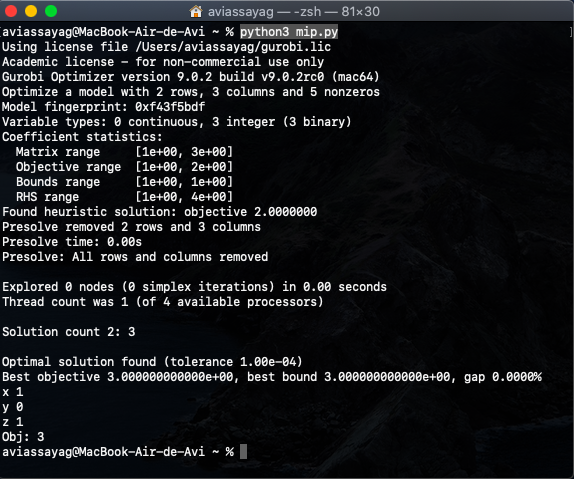
\includegraphics[scale=0.4]{gurobipython.png}
\caption{Résolution via module gurobi (gurobipy)}
\end{figure}
\end{center}
Il est logique que le résultat produit est le même sauf la commande utilisé n'est pas la même. L'avantage de la deuxième méthode est que l'on peut importer le module \textsf{gurobipy} dans n'importe quelle future création Python.
\newpage
\subsection{CV}
\begin{center}
\begin{figure}[h!]
\centering
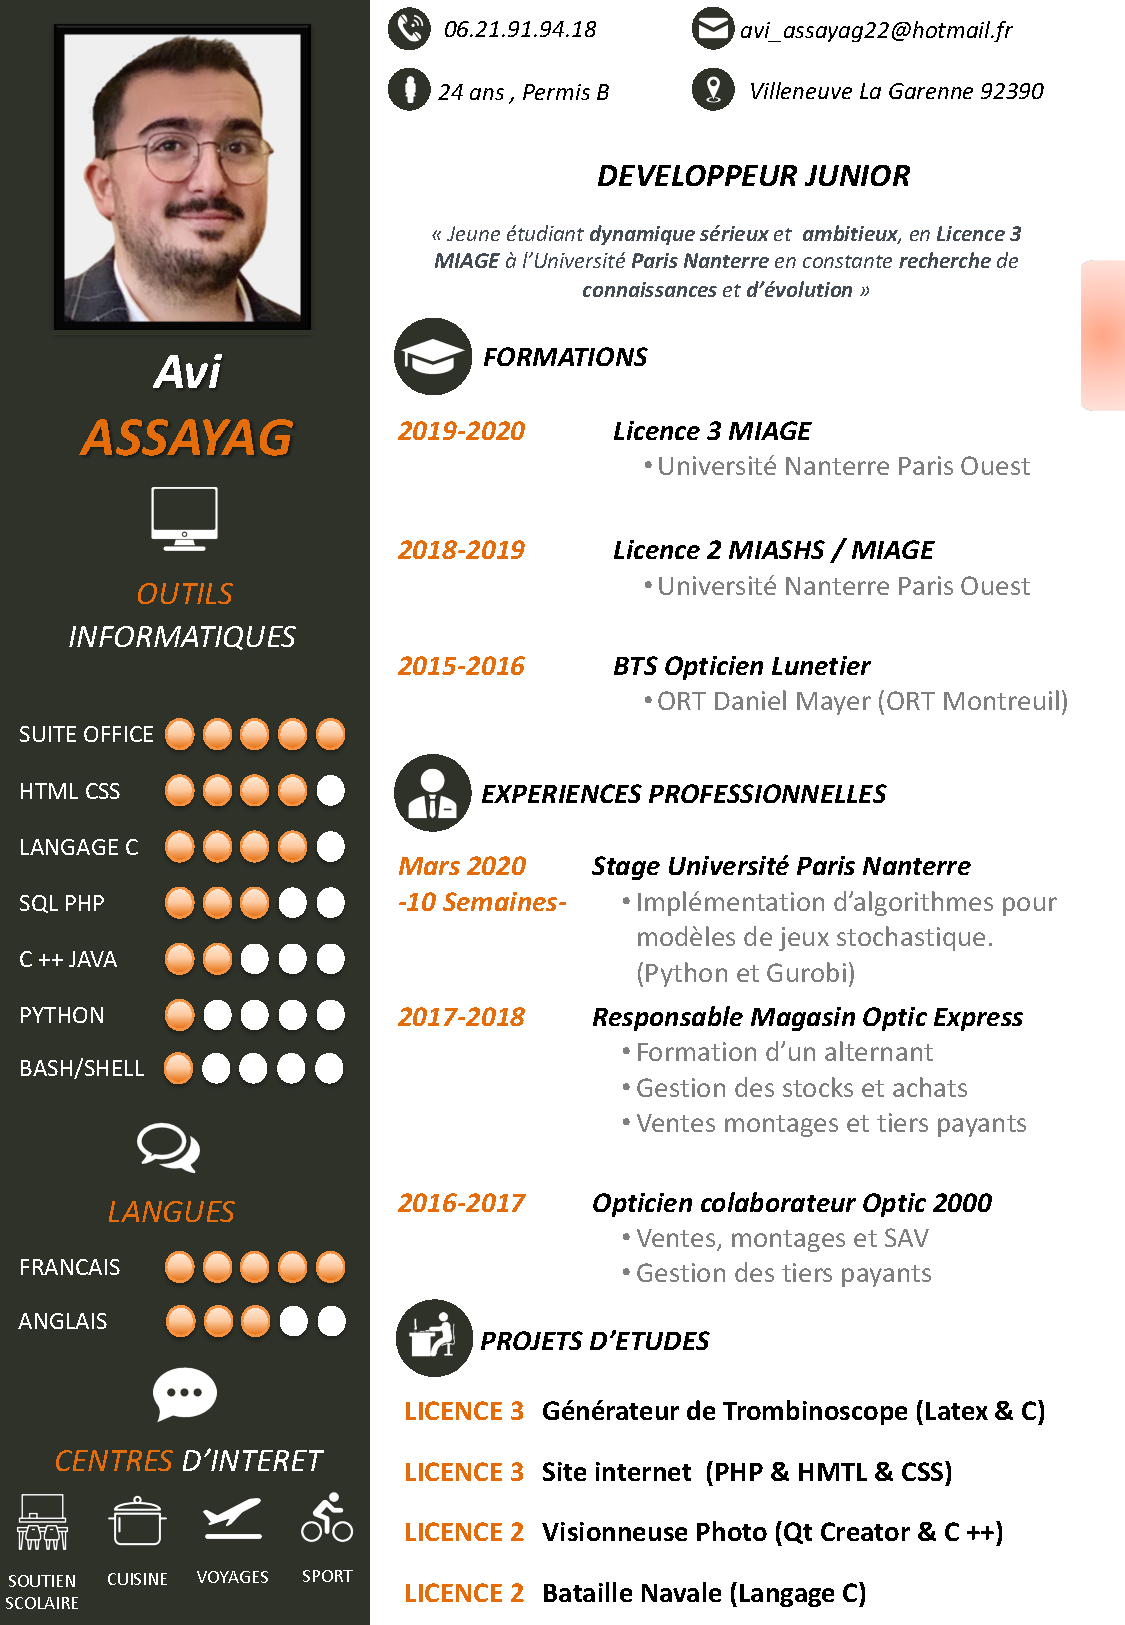
\includegraphics [scale=0.83]{CV.pdf}
\caption{Curriculum Vitae Avi ASSAYAG L3 MIAGE}
\end{figure}
\end{center}
\listoffigures\
\end{document}

